\documentclass[12pt,a4paper]{article}

\usepackage[a4paper,margin=1in]{geometry}
\usepackage{graphicx}
\usepackage{booktabs}
\usepackage{amsmath,amssymb}
\usepackage{float}
\usepackage{hyperref}
\usepackage{xcolor}
\usepackage{listings}
\usepackage{enumitem}
\usepackage{fancyhdr}
\usepackage{longtable}
\usepackage{multirow}

\hypersetup{colorlinks=true,linkcolor=blue,urlcolor=blue}

\pagestyle{fancy}
\fancyhf{}
\lhead{ICS1512}
\rhead{Machine Learning Algorithms Laboratory}
\cfoot{\thepage}

\lstset{
language=Python,
basicstyle=\ttfamily\small,
numbers=left,
frame=single,
breaklines=true,
showstringspaces=false
}

\begin{document}

\begin{tabular}{|p{4cm}|p{11cm}|}
\hline
Experiment No. & 7 \\ \hline
Experiment Title & Dimensionality Reduction and Model Evaluation (With and Without PCA) \href{https://github.com/Kavin-ks/Machine-Learning-Projects}{\textsuperscript{1}}\\ \hline
Student Name & Kavinsoorya K S \\ \hline
Register Number & 3122247001030 \\ \hline
Faculty & Dr. Poreddy Ajay Kumar Reddy \\ \hline
Submission Date & August 30, 2026 \\ \hline
\end{tabular}

\vspace{0.5cm}

\section{Objective}
The objective of this experiment is to study the effect of dimensionality reduction using Principal Component Analysis (PCA) on the classification performance of ten machine learning models. Each model is trained and evaluated under two settings: using the original standardized features (\textbf{No-PCA}) and using PCA-reduced features (\textbf{With-PCA}). Hyperparameter tuning via GridSearchCV with 5-fold stratified cross-validation is performed for all models under both conditions. The experiment compares accuracy, precision, recall, F1-score, and ROC-AUC to determine which models benefit from dimensionality reduction and which do not.

\section{Problem Statement}
Given a diagnostic dataset $\mathcal{D} = \{(\mathbf{x}_i, y_i)\}_{i=1}^{569}$ where $\mathbf{x}_i \in \mathbb{R}^{30}$ represents continuous features computed from cell nuclei measurements in breast mass biopsies and $y_i \in \{0, 1\}$ denotes the diagnostic label (0 for Malignant, 1 for Benign), the task is to:
\begin{enumerate}
    \item Standardize the feature space and apply PCA to obtain a reduced representation $\mathbf{x}_i' \in \mathbb{R}^{k}$ where $k < 30$, retaining at least 95\% of the total variance.
    \item Train ten classifiers (SVM, Na\"ive Bayes, KNN, Logistic Regression, Decision Tree, Random Forest, AdaBoost, Gradient Boosting, XGBoost, and Stacking) on both the original and PCA-reduced feature spaces.
    \item Perform hyperparameter tuning and 5-fold cross-validation for each model under both settings.
    \item Compare and analyze whether PCA improved accuracy, F1-score, or prediction stability.
\end{enumerate}

\section{Dataset Description}
The analysis uses the \textbf{Wisconsin Diagnostic Breast Cancer (WDBC)} dataset from the scikit-learn library. Table~\ref{tab:dataset_summary} summarizes the dataset characteristics.

\begin{longtable}{|p{6cm}|p{8cm}|}
\hline
Dataset Name & Wisconsin Diagnostic Breast Cancer (WDBC) Dataset \\ \hline
Dataset Source & scikit-learn (\texttt{sklearn.datasets.load\_breast\_cancer}) \\ \hline
Number of Samples & 569 \\ \hline
Number of Features & 30 continuous numerical attributes \\ \hline
Number of Classes & 2 (Malignant: 0, Benign: 1) \\ \hline
Missing Values & 0 (complete dataset) \\ \hline
Duplicate Rows & 0 \\ \hline
Train-Test Split & 80\% Training (455) / 20\% Testing (114) \\ \hline
Training Class Distribution & Benign (1): 285 (62.64\%), Malignant (0): 170 (37.36\%) \\ \hline
Testing Class Distribution & Benign (1): 72 (63.16\%), Malignant (0): 42 (36.84\%) \\ \hline
\label{tab:dataset_summary}
\end{longtable}

The 30 features describe ten physical properties of cell nuclei (radius, texture, perimeter, area, smoothness, compactness, concavity, concave points, symmetry, fractal dimension), each summarized by three statistics: mean, standard error, and worst (mean of the three largest values).

\section{Exploratory Data Analysis}

\subsection{Class Distribution}
\begin{figure}[H]
\centering

\includegraphics[width=0.55\linewidth]{images/class_distribution.png}
\caption{Class Distribution of Malignant (0) vs. Benign (1) Samples}
\label{fig:class_dist}
\end{figure}

\textbf{Inference:}
The dataset contains 357 benign samples (62.74\%) and 212 malignant samples (37.26\%), indicating moderate class imbalance. Stratified sampling was used during the train-test split to preserve this distribution in both the training set (285 Benign, 170 Malignant) and testing set (72 Benign, 42 Malignant). This prevents models from developing bias toward the majority class.

\subsection{Feature Correlation Analysis}
\begin{figure}[H]
\centering

\includegraphics[width=0.75\linewidth]{images/correlation_heatmap.png}
\caption{Pairwise Correlation Heatmap of 30 Features (Lower Triangle)}
\label{fig:corr_heatmap}
\end{figure}

\textbf{Inference:}
The heatmap reveals high multicollinearity among several feature groups, particularly radius, perimeter, and area variants (Pearson coefficients approaching 1.0). This strong redundancy across features makes the dataset well-suited for PCA, which can compress correlated variables into fewer orthogonal components. For linear models like Logistic Regression, multicollinearity can cause coefficient instability, so PCA's decorrelation effect is expected to benefit them.

\section{Data Preprocessing}
The preprocessing pipeline consists of:
\begin{enumerate}
    \item \textbf{Feature-Target Separation}: The 30 numerical features were separated from the binary target variable.
    \item \textbf{Train-Test Split}: An 80-20 stratified split was applied using \texttt{random\_state=42} to ensure reproducibility and class balance.
    \item \textbf{Standardization}: \texttt{StandardScaler} was fitted on the training set and applied to both training and testing sets to prevent data leakage. After scaling, training features have zero mean and unit variance.
    \item \textbf{PCA}: Applied to the standardized training features (details in the PCA Design section).
\end{enumerate}

\begin{lstlisting}[caption={Preprocessing and PCA Pipeline}]
scaler = StandardScaler()
X_train_scaled = scaler.fit_transform(X_train)
X_test_scaled = scaler.transform(X_test)

pca = PCA(n_components=0.95, random_state=42)
X_train_pca = pca.fit_transform(X_train_scaled)
X_test_pca = pca.transform(X_test_scaled)
\end{lstlisting}

\section{PCA Design}

PCA was applied with a 95\% variance retention threshold, fitted only on the training data. This resulted in \textbf{10 principal components} (out of 30 original features) capturing \textbf{95.27\%} of the total variance.

\begin{table}[H]
\centering
\caption{PCA Variance Summary}
\label{tab:pca_summary}
\vspace{0.2cm}
\begin{tabular}{llll}
\toprule
\textbf{Setting} & \textbf{Components} & \textbf{Variance (\%)} & \textbf{Justification} \\
\midrule
With-PCA & 10 (95\% target) & 95.27\% & Retain maximum information with minimum dimensions \\
\bottomrule
\end{tabular}
\end{table}

\begin{table}[H]
\centering
\caption{Component-wise Explained Variance}
\label{tab:pca_components}
\vspace{0.2cm}
\begin{tabular}{lcc}
\toprule
\textbf{Component} & \textbf{Individual (\%)} & \textbf{Cumulative (\%)} \\
\midrule
PC1 & 44.41 & 44.41 \\
PC2 & 18.94 & 63.36 \\
PC3 & 9.54 & 72.90 \\
PC4 & 6.72 & 79.63 \\
PC5 & 5.52 & 85.14 \\
PC6 & 3.93 & 89.08 \\
PC7 & 2.18 & 91.26 \\
PC8 & 1.58 & 92.84 \\
PC9 & 1.28 & 94.12 \\
PC10 & 1.15 & 95.27 \\
\bottomrule
\end{tabular}
\end{table}

\subsection{Scree Plot}
\begin{figure}[H]
\centering
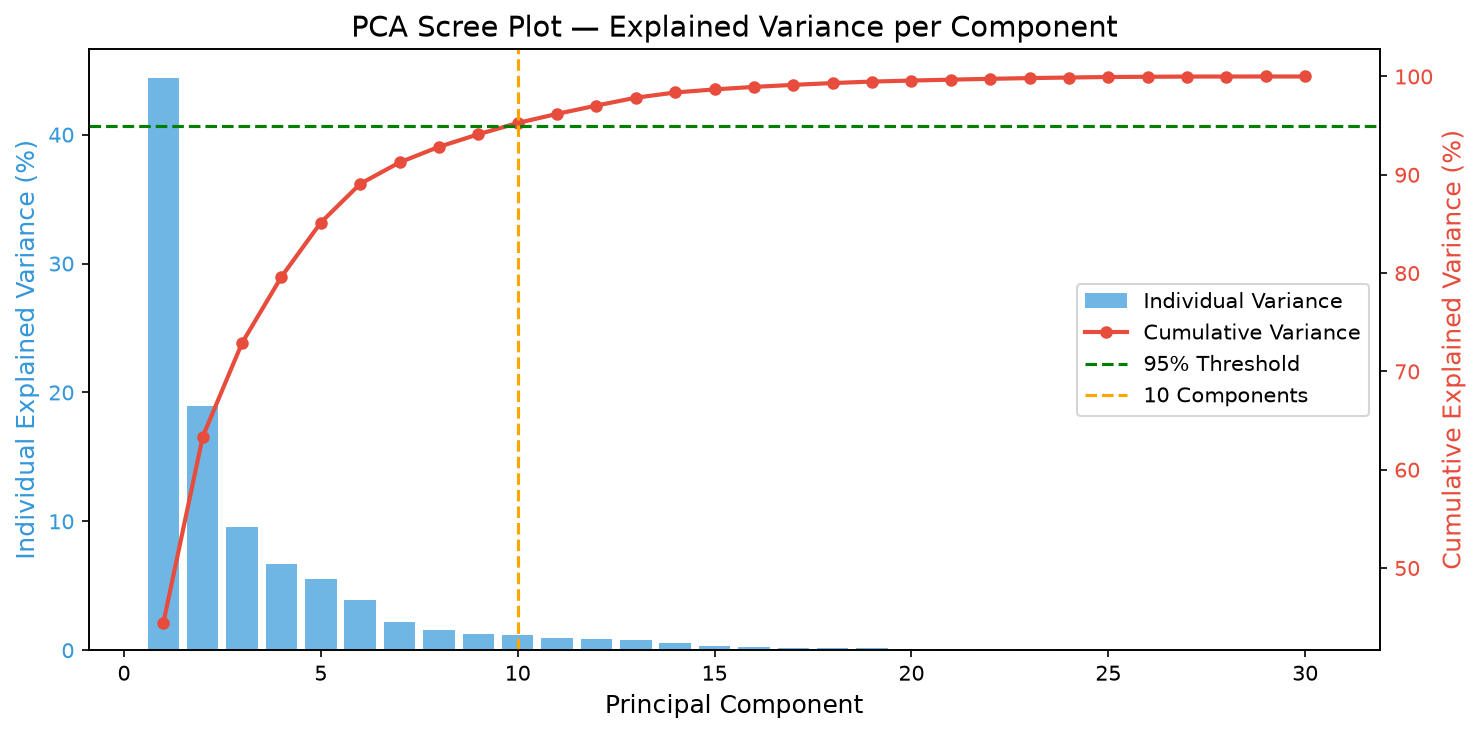
\includegraphics[width=0.75\linewidth]{images/pca_scree_plot.png}
\caption{PCA Scree Plot — Individual and Cumulative Explained Variance}
\label{fig:scree}
\end{figure}

\textbf{Inference:}
The first principal component alone captures 44.41\% of the variance, and the first three components account for 72.90\%. The curve flattens after approximately 10 components, confirming that the remaining 20 components contribute minimal information. The 95\% threshold line intersects the cumulative curve at 10 components, validating the chosen retention target.

\section{Machine Learning Algorithm}

\subsection{Principal Component Analysis (PCA)}
\textbf{Working Principle:} PCA is a linear dimensionality reduction technique that transforms the original feature space into a new set of orthogonal axes (principal components) ordered by the amount of variance they capture. By projecting the data onto the top $k$ components, PCA reduces dimensionality while preserving the maximum possible variance.\\
\textbf{Mathematical Formulation:}
Given a centered data matrix $\mathbf{X} \in \mathbb{R}^{n \times p}$, PCA computes the covariance matrix $\mathbf{C} = \frac{1}{n-1}\mathbf{X}^T\mathbf{X}$ and performs eigendecomposition $\mathbf{C} = \mathbf{V}\mathbf{\Lambda}\mathbf{V}^T$, where $\mathbf{V}$ contains the eigenvectors (principal directions) and $\mathbf{\Lambda}$ contains the eigenvalues (variance along each direction). The reduced representation is $\mathbf{Z} = \mathbf{X}\mathbf{V}_k$, where $\mathbf{V}_k \in \mathbb{R}^{p \times k}$ contains the top $k$ eigenvectors.\\
\textbf{Advantages:} Removes multicollinearity, reduces noise, lowers computational cost.\\
\textbf{Limitations:} Linear transformation only, components lose feature interpretability.

\subsection{Classifiers}
The following ten classifiers were evaluated:
\begin{enumerate}
    \item \textbf{SVM}: Maximum-margin hyperplane classifier with kernel transformations.
    \item \textbf{Na\"ive Bayes}: Probabilistic classifier using Bayes' theorem with feature independence assumption.
    \item \textbf{KNN}: Instance-based learner classifying by majority vote among $k$ nearest neighbors.
    \item \textbf{Logistic Regression}: Linear model using sigmoid function for probabilistic classification.
    \item \textbf{Decision Tree}: Recursive axis-aligned partitioning of the feature space.
    \item \textbf{Random Forest}: Ensemble of decision trees trained on bootstrap samples with random feature subsets.
    \item \textbf{AdaBoost}: Sequential boosting with weighted weak learners focusing on misclassified samples.
    \item \textbf{Gradient Boosting}: Sequential boosting minimizing a differentiable loss function via pseudo-residuals.
    \item \textbf{XGBoost}: Regularized gradient boosting with built-in L1/L2 regularization and efficient implementation.
    \item \textbf{Stacking}: Heterogeneous ensemble combining diverse base learners through a meta-learner.
\end{enumerate}

\section{Experimental Setup}

\begin{table}[H]
\centering
\caption{Experimental Setup Specifications}
\label{tab:exp_setup}
\vspace{0.2cm}
\begin{tabular}{ll}
\toprule
\textbf{Parameter} & \textbf{Specification} \\
\midrule
Python Version & 3.13 \\
Scikit-Learn Version & 1.9.0 \\
XGBoost Version & 3.0+ \\
IDE & Jupyter Notebook \\
Operating System & macOS Sequoia \\
Hardware & Apple Silicon M-Series / 16 GB Unified Memory \\
\bottomrule
\end{tabular}
\end{table}

\section{Hyperparameter Selection}

Hyperparameter tuning was performed for all 10 models under both No-PCA and With-PCA settings using GridSearchCV with 5-fold stratified cross-validation.

\subsection{SVM}

\begin{longtable}{|c|c|c|c|c|}
\hline
\textbf{Kernel} & \textbf{C} & \textbf{Gamma} & \textbf{Perf. (No-PCA)} & \textbf{Perf. (With-PCA)} \\ \hline
\endhead
linear & 0.1 & scale & 0.9758 & 0.9714 \\ \hline
linear & 0.1 & auto & 0.9758 & 0.9714 \\ \hline
linear & 1 & scale & 0.9714 & 0.9780 \\ \hline
linear & 1 & auto & 0.9714 & 0.9780 \\ \hline
linear & 10 & scale & 0.9670 & 0.9736 \\ \hline
linear & 10 & auto & 0.9670 & 0.9736 \\ \hline
rbf & 0.1 & scale & 0.9582 & 0.9582 \\ \hline
rbf & 0.1 & auto & 0.9209 & 0.9560 \\ \hline
rbf & 1 & scale & 0.9758 & 0.9758 \\ \hline
rbf & 1 & auto & 0.9560 & 0.9736 \\ \hline
rbf & 10 & scale & 0.9714 & 0.9692 \\ \hline
rbf & 10 & auto & 0.9604 & 0.9670 \\ \hline
\caption{SVM — Hyperparameter Tuning Results}
\label{tab:svm_tuning}
\end{longtable}

\textbf{Best Parameters (No-PCA):} kernel=linear, C=0.1, gamma=scale (CV Accuracy: 97.58\%)\\
\textbf{Best Parameters (With-PCA):} kernel=linear, C=1, gamma=scale (CV Accuracy: 97.80\%)

\subsection{Na\"ive Bayes}

\begin{longtable}{|c|c|c|}
\hline
\textbf{Smoothing Parameter} & \textbf{Perf. (No-PCA)} & \textbf{Perf. (With-PCA)} \\ \hline
\endhead
1e-11 & 0.9341 & 0.9165 \\ \hline
1e-10 & 0.9341 & 0.9165 \\ \hline
1e-09 & 0.9341 & 0.9165 \\ \hline
1e-08 & 0.9297 & 0.9165 \\ \hline
1e-07 & 0.9297 & 0.9165 \\ \hline
1e-06 & 0.9297 & 0.9143 \\ \hline
1e-05 & 0.9275 & 0.9077 \\ \hline
\caption{Na\"ive Bayes — Smoothing Choices}
\label{tab:nb_tuning}
\end{longtable}

\textbf{Best Parameters (No-PCA):} var\_smoothing=1e-11 (CV Accuracy: 93.41\%)\\
\textbf{Best Parameters (With-PCA):} var\_smoothing=1e-11 (CV Accuracy: 91.65\%)

\subsection{KNN}

\begin{longtable}{|c|c|c|c|c|}
\hline
\textbf{k} & \textbf{Weights} & \textbf{Metric} & \textbf{Perf. (No-PCA)} & \textbf{Perf. (With-PCA)} \\ \hline
\endhead
3 & uniform & manhattan & 0.9714 & 0.9648 \\ \hline
5 & uniform & euclidean & 0.9670 & 0.9648 \\ \hline
5 & uniform & manhattan & 0.9670 & 0.9560 \\ \hline
3 & uniform & euclidean & 0.9648 & 0.9604 \\ \hline
3 & distance & manhattan & 0.9648 & 0.9604 \\ \hline
\caption{KNN — Hyperparameter Tuning (Top 5)}
\label{tab:knn_tuning}
\end{longtable}

\textbf{Best Parameters (No-PCA):} k=3, weights=uniform, metric=manhattan (CV Accuracy: 97.14\%)\\
\textbf{Best Parameters (With-PCA):} k=5, weights=uniform, metric=euclidean (CV Accuracy: 96.48\%)

\subsection{Logistic Regression}

\begin{longtable}{|c|c|c|c|c|}
\hline
\textbf{C} & \textbf{Penalty} & \textbf{Solver} & \textbf{Perf. (No-PCA)} & \textbf{Perf. (With-PCA)} \\ \hline
\endhead
0.01 & l2 & lbfgs & 0.9780 & 0.9802 \\ \hline
0.1 & l2 & lbfgs & 0.9824 & 0.9824 \\ \hline
1 & l2 & lbfgs & 0.9802 & 0.9802 \\ \hline
10 & l2 & lbfgs & 0.9736 & 0.9802 \\ \hline
100 & l2 & lbfgs & 0.9736 & 0.9780 \\ \hline
\caption{Logistic Regression — Hyperparameter Tuning}
\label{tab:lr_tuning}
\end{longtable}

\textbf{Best Parameters (No-PCA):} C=0.1 (CV Accuracy: 98.24\%)\\
\textbf{Best Parameters (With-PCA):} C=0.1 (CV Accuracy: 98.24\%)

\subsection{Decision Tree}

\begin{longtable}{|c|c|c|c|c|}
\hline
\textbf{Max Depth} & \textbf{Min Split} & \textbf{Criterion} & \textbf{Perf. (No-PCA)} & \textbf{Perf. (With-PCA)} \\ \hline
\endhead
3 & 2 & entropy & 0.9319 & 0.9297 \\ \hline
5 & 10 & entropy & 0.9297 & 0.9385 \\ \hline
3 & 5 & entropy & 0.9297 & 0.9297 \\ \hline
5 & 2 & gini & 0.9275 & 0.9275 \\ \hline
7 & 5 & gini & 0.9275 & 0.9275 \\ \hline
\caption{Decision Tree — Hyperparameter Tuning (Top 5)}
\label{tab:dt_tuning}
\end{longtable}

\textbf{Best Parameters (No-PCA):} criterion=entropy, max\_depth=3, min\_samples\_split=2 (CV Accuracy: 93.19\%)\\
\textbf{Best Parameters (With-PCA):} criterion=entropy, max\_depth=5, min\_samples\_split=10 (CV Accuracy: 93.85\%)

\subsection{Random Forest}

\begin{longtable}{|c|c|c|c|c|}
\hline
\textbf{N Est.} & \textbf{Max Depth} & \textbf{Min Split} & \textbf{Perf. (No-PCA)} & \textbf{Perf. (With-PCA)} \\ \hline
\endhead
200 & 5 & 5 & 0.9626 & 0.9560 \\ \hline
100 & 5 & 5 & 0.9626 & 0.9538 \\ \hline
50 & 5 & 5 & 0.9604 & 0.9516 \\ \hline
200 & 10 & 2 & 0.9604 & 0.9582 \\ \hline
200 & None & 2 & 0.9604 & 0.9604 \\ \hline
\caption{Random Forest — Hyperparameter Tuning (Top 5)}
\label{tab:rf_tuning}
\end{longtable}

\textbf{Best Parameters (No-PCA):} n\_estimators=200, max\_depth=5, min\_split=5 (CV Accuracy: 96.26\%)\\
\textbf{Best Parameters (With-PCA):} n\_estimators=200, max\_depth=None, min\_split=2 (CV Accuracy: 96.04\%)

\subsection{AdaBoost}

\begin{longtable}{|c|c|c|c|c|}
\hline
\textbf{N Est.} & \textbf{LR} & \textbf{Depth} & \textbf{Perf. (No-PCA)} & \textbf{Perf. (With-PCA)} \\ \hline
\endhead
100 & 1.0 & 1 & 0.9802 & 0.9670 \\ \hline
50 & 1.0 & 1 & 0.9780 & 0.9626 \\ \hline
200 & 1.0 & 1 & 0.9780 & 0.9692 \\ \hline
200 & 0.5 & 1 & 0.9758 & 0.9626 \\ \hline
200 & 0.5 & 3 & 0.9714 & 0.9714 \\ \hline
\caption{AdaBoost — Hyperparameter Tuning (Top 5)}
\label{tab:ada_tuning}
\end{longtable}

\textbf{Best Parameters (No-PCA):} n\_estimators=100, learning\_rate=1.0, max\_depth=1 (CV Accuracy: 98.02\%)\\
\textbf{Best Parameters (With-PCA):} n\_estimators=200, learning\_rate=0.5, max\_depth=3 (CV Accuracy: 97.14\%)

\subsection{Gradient Boosting}

\begin{longtable}{|c|c|c|c|c|}
\hline
\textbf{N Est.} & \textbf{LR} & \textbf{Depth} & \textbf{Perf. (No-PCA)} & \textbf{Perf. (With-PCA)} \\ \hline
\endhead
200 & 0.2 & 3 & 0.9736 & 0.9626 \\ \hline
100 & 0.2 & 3 & 0.9714 & 0.9604 \\ \hline
200 & 0.1 & 3 & 0.9692 & 0.9626 \\ \hline
100 & 0.1 & 3 & 0.9670 & 0.9604 \\ \hline
200 & 0.2 & 5 & 0.9670 & 0.9604 \\ \hline
\caption{Gradient Boosting — Hyperparameter Tuning (Top 5)}
\label{tab:gb_tuning}
\end{longtable}

\textbf{Best Parameters (No-PCA):} n\_estimators=200, learning\_rate=0.2, max\_depth=3 (CV Accuracy: 97.36\%)\\
\textbf{Best Parameters (With-PCA):} n\_estimators=200, learning\_rate=0.1, max\_depth=3 (CV Accuracy: 96.26\%)

\subsection{XGBoost}

\begin{longtable}{|c|c|c|c|c|c|}
\hline
\textbf{N Est.} & \textbf{LR} & \textbf{Depth} & \textbf{Sub.} & \textbf{Perf. (NP)} & \textbf{Perf. (WP)} \\ \hline
\endhead
100 & 0.1 & 3 & 1.0 & 0.9714 & 0.9648 \\ \hline
100 & 0.1 & 3 & 0.8 & 0.9714 & 0.9604 \\ \hline
200 & 0.1 & 3 & 1.0 & 0.9714 & 0.9626 \\ \hline
200 & 0.1 & 3 & 0.8 & 0.9692 & 0.9670 \\ \hline
100 & 0.2 & 3 & 1.0 & 0.9692 & 0.9516 \\ \hline
\caption{XGBoost — Hyperparameter Tuning (Top 5)}
\label{tab:xgb_tuning}
\end{longtable}

\textbf{Best Parameters (No-PCA):} n\_estimators=100, learning\_rate=0.1, max\_depth=3, subsample=1.0 (CV Accuracy: 97.14\%)\\
\textbf{Best Parameters (With-PCA):} n\_estimators=200, learning\_rate=0.1, max\_depth=5, subsample=0.8 (CV Accuracy: 96.70\%)

\subsection{Stacking}

\begin{longtable}{|p{5cm}|p{3cm}|c|c|}
\hline
\textbf{Base Models} & \textbf{Meta Learner} & \textbf{CV Acc (NP)} & \textbf{CV Acc (WP)} \\ \hline
\endhead
SVM, Na\"ive Bayes, KNN, Decision Tree, Random Forest & Logistic Regression & 97.14\% & 97.58\% \\ \hline
\caption{Stacking Classifier — Configuration and CV Performance}
\label{tab:stk_tuning}
\end{longtable}

The best hyperparameters from each model's individual tuning were used for the Stacking base estimators. The meta-learner (Logistic Regression, max\_iter=5000) combines the out-of-fold predictions of the five base classifiers.

\section{Results}

\subsection{5-Fold Cross-Validation (No-PCA vs With-PCA)}

\begin{longtable}{|l|c|c|c|c|c|c|c|}
\hline
\textbf{Model} & \textbf{F1} & \textbf{F2} & \textbf{F3} & \textbf{F4} & \textbf{F5} & \textbf{Avg (NP)} & \textbf{Avg (WP)} \\ \hline
\endhead
SVM & 0.9560 & 0.9780 & 0.9780 & 0.9780 & 0.9890 & 0.9758 & 0.9780 \\ \hline
Na\"ive Bayes & 0.9121 & 0.9670 & 0.8901 & 0.9560 & 0.9451 & 0.9341 & 0.9165 \\ \hline
KNN & 0.9780 & 0.9890 & 0.9560 & 0.9560 & 0.9780 & 0.9714 & 0.9648 \\ \hline
Log. Regression & 0.9780 & 0.9780 & 0.9890 & 0.9780 & 0.9890 & 0.9824 & 0.9824 \\ \hline
Decision Tree & 0.9011 & 0.9451 & 0.9121 & 0.9341 & 0.9670 & 0.9319 & 0.9385 \\ \hline
Random Forest & 0.9560 & 0.9670 & 0.9341 & 0.9670 & 0.9890 & 0.9626 & 0.9604 \\ \hline
AdaBoost & 0.9890 & 1.0000 & 0.9451 & 0.9780 & 0.9890 & 0.9802 & 0.9714 \\ \hline
Grad. Boosting & 0.9780 & 0.9890 & 0.9560 & 0.9560 & 0.9890 & 0.9736 & 0.9626 \\ \hline
XGBoost & 0.9890 & 0.9780 & 0.9451 & 0.9560 & 0.9890 & 0.9714 & 0.9670 \\ \hline
Stacking & 0.9670 & 0.9780 & 0.9451 & 0.9780 & 0.9890 & 0.9714 & 0.9758 \\ \hline
\caption{5-Fold Cross-Validation Accuracy (No-PCA Fold Scores Shown)}
\label{tab:cv_results}
\end{longtable}

\subsection{Test Performance Comparison}

\begin{table}[H]
\centering
\caption{Test Performance — No-PCA vs With-PCA}
\label{tab:test_results}
\vspace{0.2cm}
\small
\begin{tabular}{l|ccccc|ccccc}
\toprule
& \multicolumn{5}{c|}{\textbf{No-PCA}} & \multicolumn{5}{c}{\textbf{With-PCA}} \\
\textbf{Model} & \textbf{Acc} & \textbf{Prec} & \textbf{Rec} & \textbf{F1} & \textbf{AUC} & \textbf{Acc} & \textbf{Prec} & \textbf{Rec} & \textbf{F1} & \textbf{AUC} \\
\midrule
SVM & .9825 & .9861 & .9861 & .9861 & .9937 & .9649 & .9857 & .9583 & .9718 & .9950 \\
Na\"ive Bayes & .9298 & .9444 & .9444 & .9444 & .9868 & .9211 & .9315 & .9444 & .9379 & .9709 \\
KNN & .9649 & .9595 & .9861 & .9726 & .9714 & .9561 & .9589 & .9722 & .9655 & .9788 \\
Log. Reg. & .9737 & .9726 & .9861 & .9793 & .9957 & .9737 & .9726 & .9861 & .9793 & .9954 \\
Dec. Tree & .9474 & .9459 & .9722 & .9589 & .9448 & .9298 & .9444 & .9444 & .9444 & .9426 \\
Rand. Forest & .9561 & .9589 & .9722 & .9655 & .9927 & .9386 & .9577 & .9444 & .9510 & .9864 \\
AdaBoost & .9561 & .9467 & .9861 & .9660 & .9818 & .9649 & .9722 & .9722 & .9722 & .9931 \\
Grad. Boost & .9561 & .9467 & .9861 & .9660 & .9957 & .9561 & .9467 & .9861 & .9660 & .9878 \\
XGBoost & .9474 & .9459 & .9722 & .9589 & .9934 & .9474 & .9583 & .9583 & .9583 & .9911 \\
Stacking & .9649 & .9595 & .9861 & .9726 & .9940 & .9561 & .9718 & .9583 & .9650 & .9911 \\
\bottomrule
\end{tabular}
\end{table}

\textbf{Best Model (No-PCA):} SVM — Accuracy: 98.25\%, F1: 0.9861, AUC: 0.9937\\
\textbf{Best Model (With-PCA):} Logistic Regression — Accuracy: 97.37\%, F1: 0.9793, AUC: 0.9954

\section{Result Visualization}

\subsection{Confusion Matrices — No-PCA}
\begin{figure}[H]
\centering
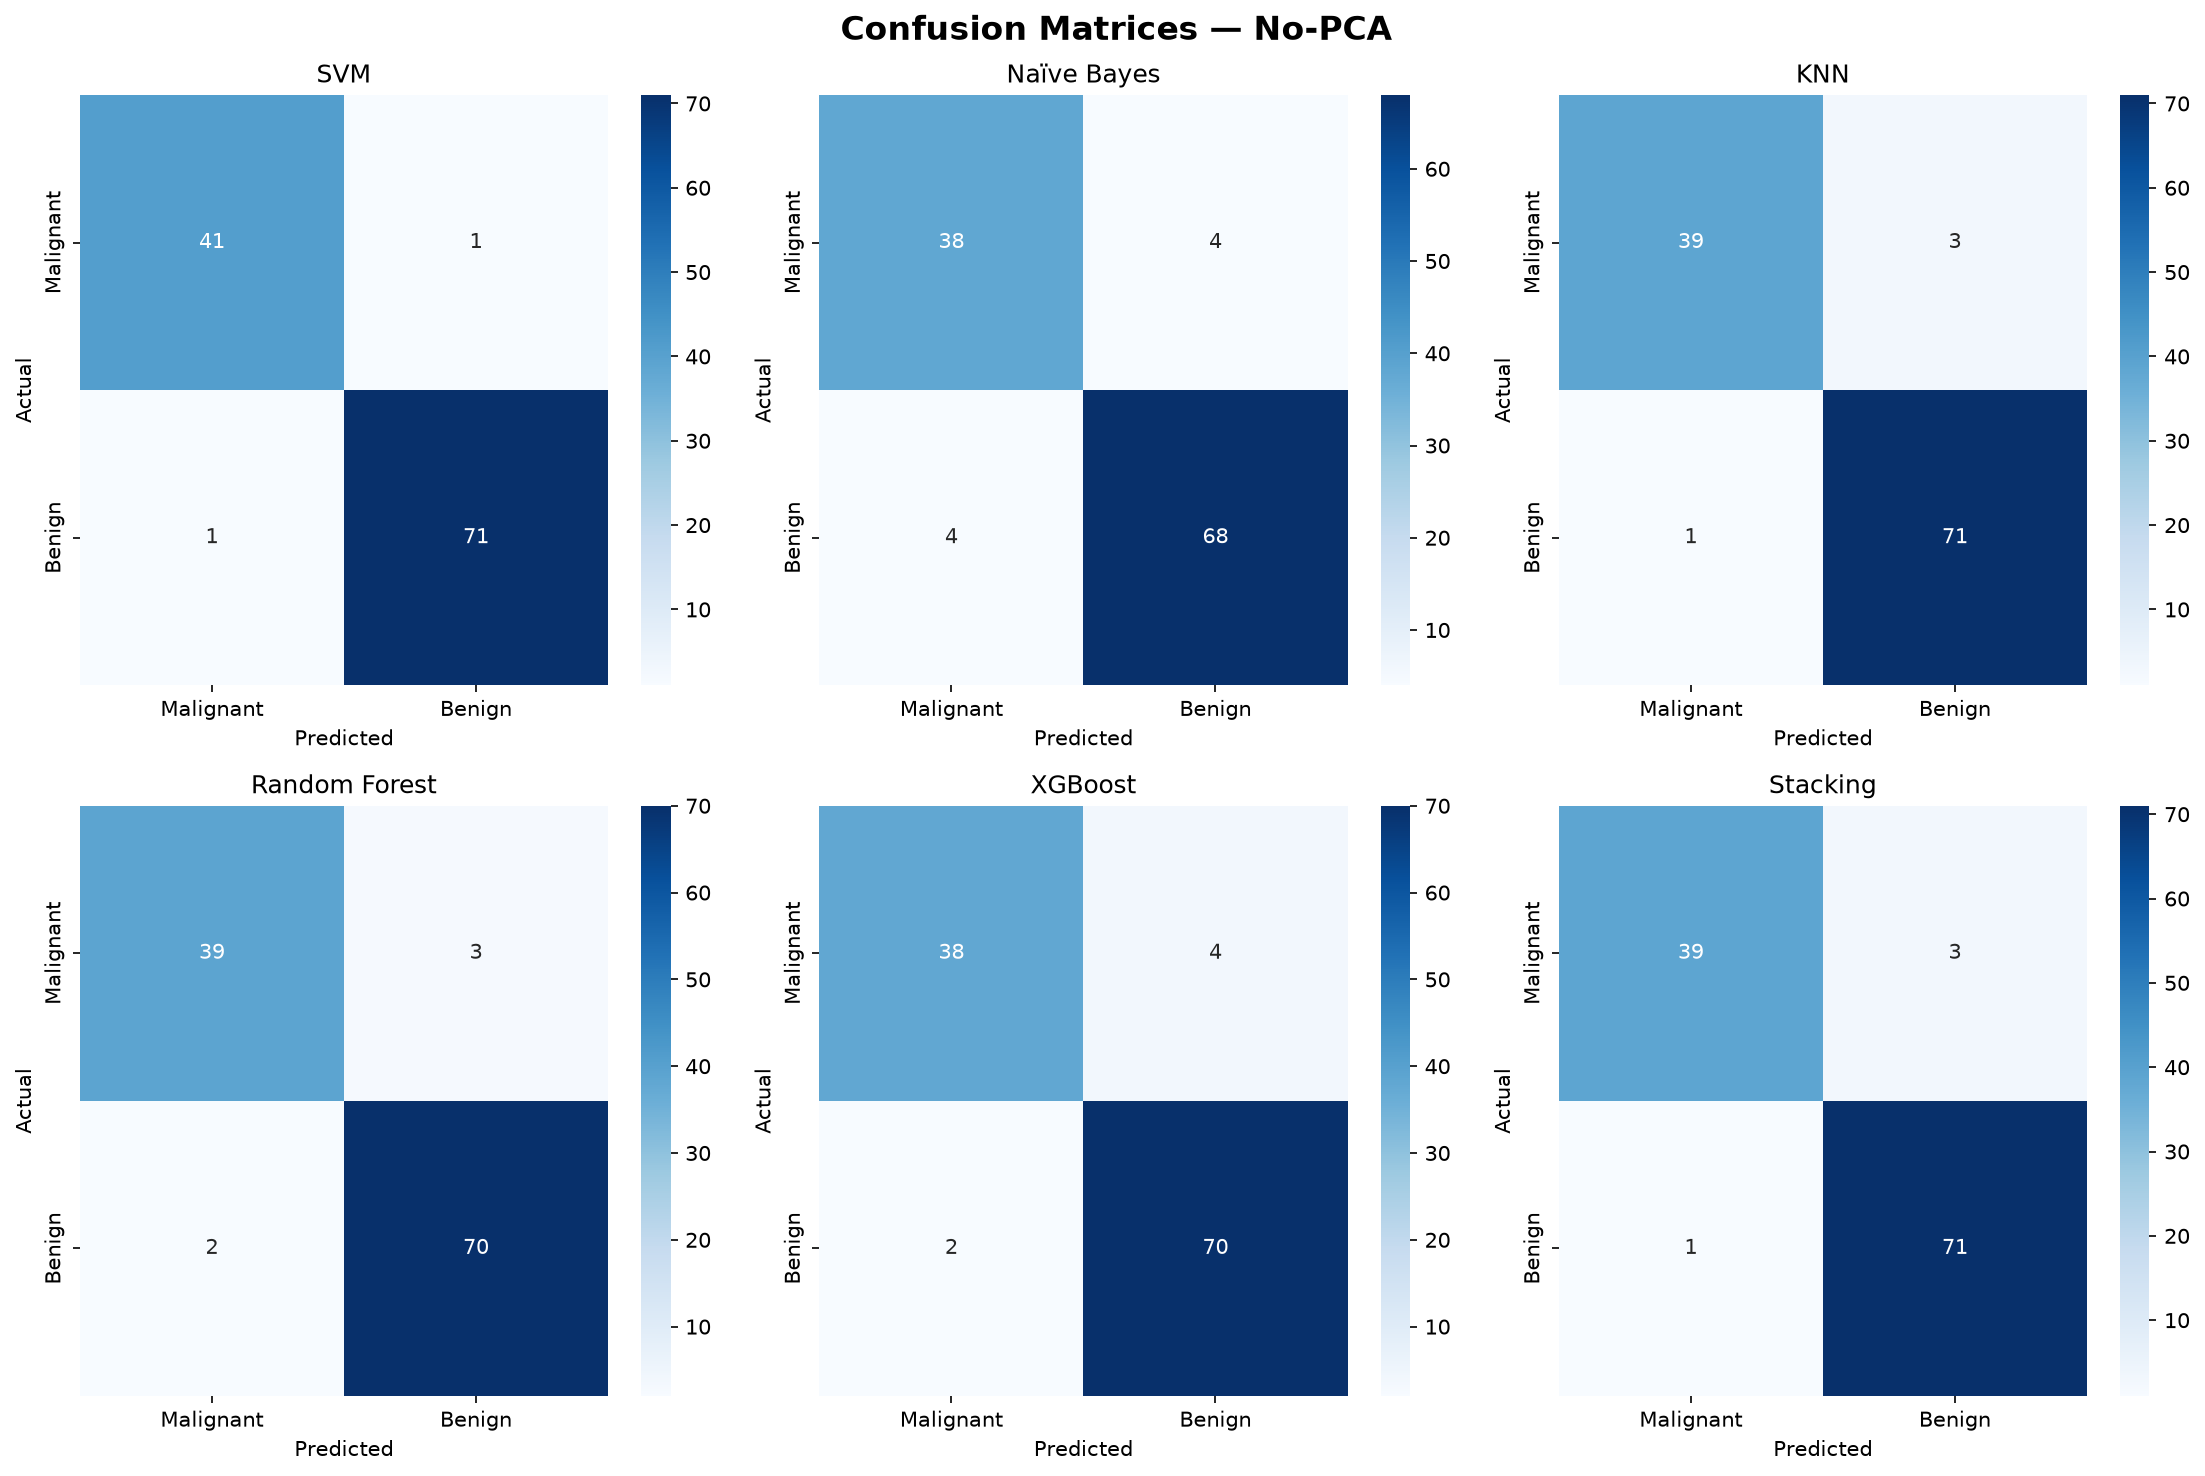
\includegraphics[width=0.9\linewidth]{images/confusion_matrices_nopca.png}
\caption{Confusion Matrices for Selected Models (No-PCA)}
\label{fig:cm_nopca}
\end{figure}

\textbf{Inference:}
The No-PCA confusion matrices show that SVM, KNN, and Stacking achieve very few misclassifications on the test set. SVM records the fewest total errors, with most models achieving high true positive rates for the benign class. The pattern of false negatives and false positives varies across model types, reflecting their different decision boundary characteristics.

\subsection{Confusion Matrices — With-PCA}
\begin{figure}[H]
\centering
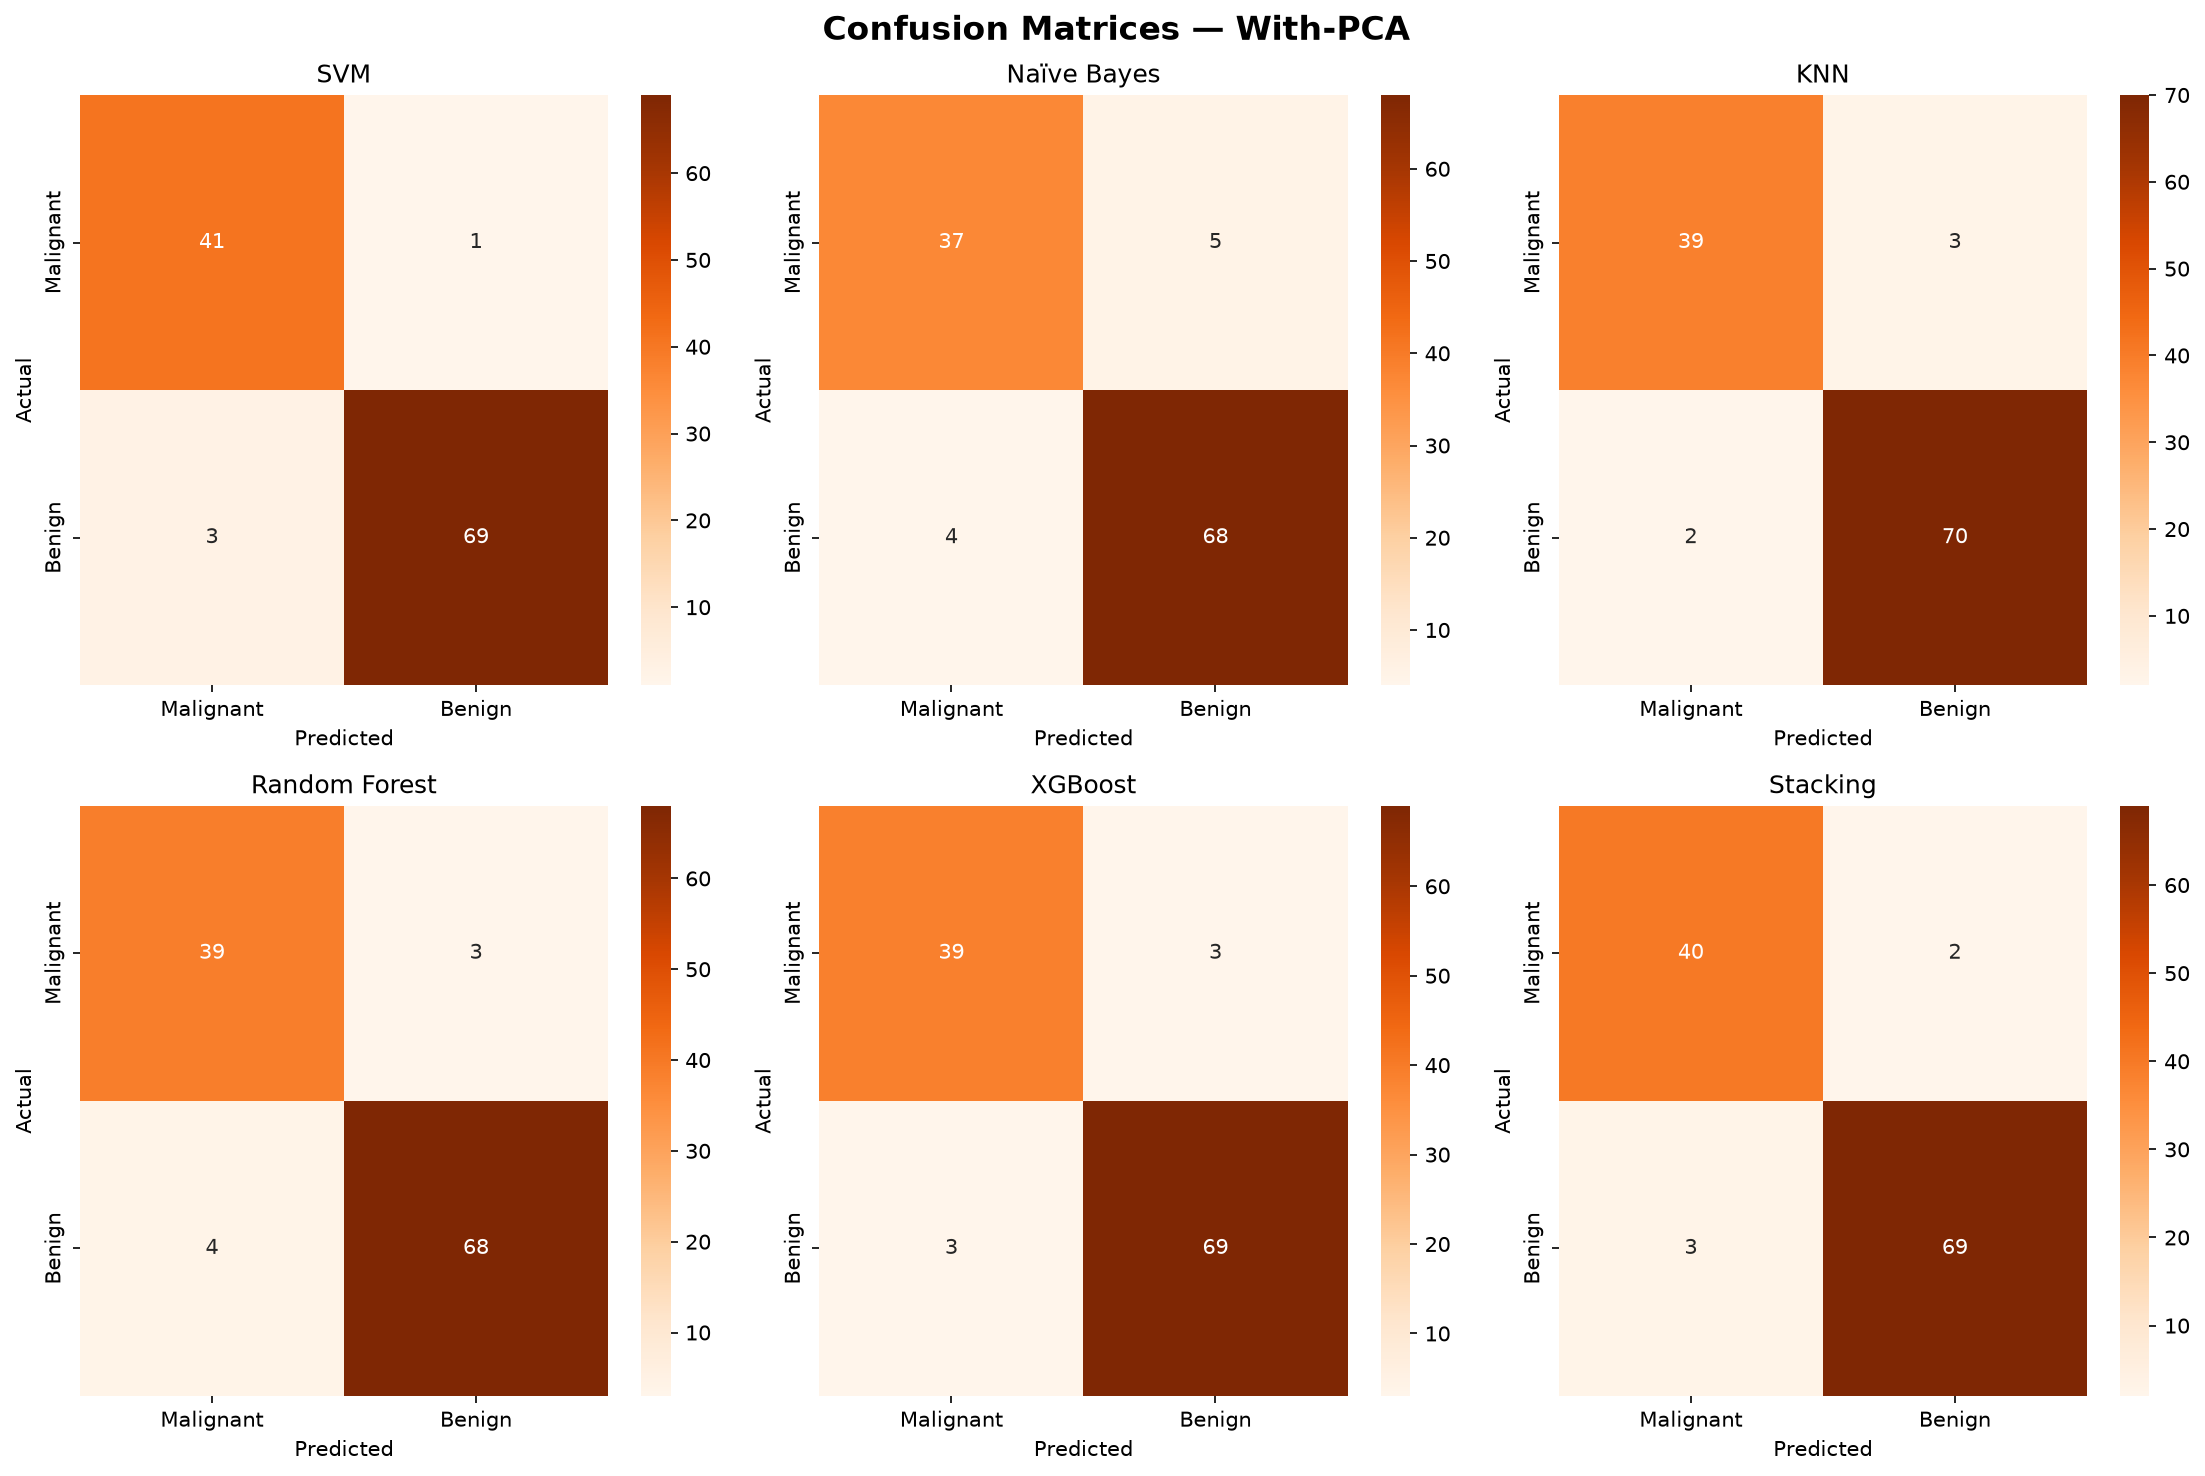
\includegraphics[width=0.9\linewidth]{images/confusion_matrices_pca.png}
\caption{Confusion Matrices for Selected Models (With-PCA)}
\label{fig:cm_pca}
\end{figure}

\textbf{Inference:}
After PCA, most models show a slight increase in misclassifications compared to their No-PCA counterparts, consistent with the small information loss from dimensionality reduction. However, AdaBoost shows improvement with PCA, suggesting that the reduced feature space helped its sequential learning process focus on more informative directions.

\subsection{ROC Curves}
\begin{figure}[H]
\centering
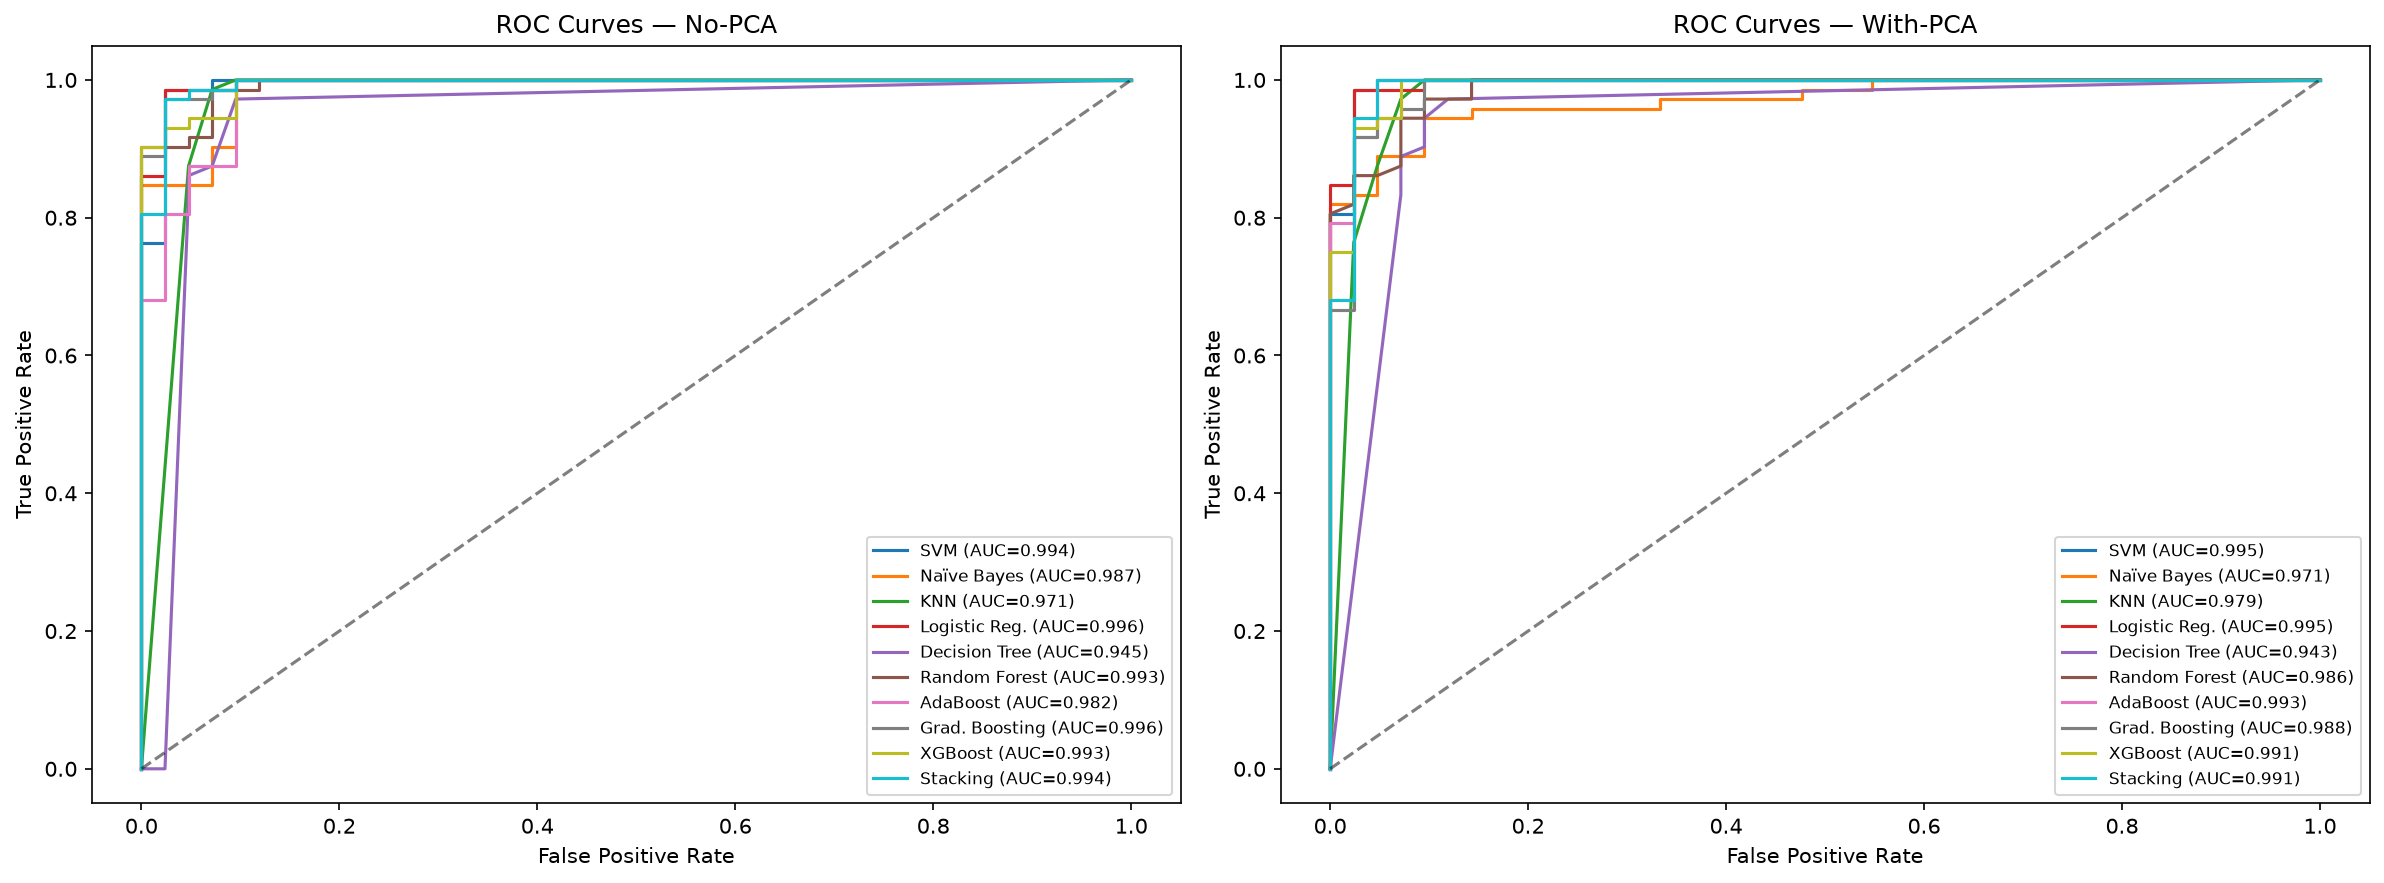
\includegraphics[width=0.95\linewidth]{images/roc_curves_comparison.png}
\caption{ROC Curve Comparison — No-PCA (Left) vs With-PCA (Right)}
\label{fig:roc}
\end{figure}

\textbf{Inference:}
The ROC curves demonstrate that all models achieve high AUC values ($>0.94$) under both settings. Logistic Regression and Gradient Boosting consistently maintain the highest AUC values. The With-PCA curves are slightly closer together, indicating that PCA narrows the performance gap between models by providing a more standardized feature representation.

\subsection{Precision-Recall Curves}
\begin{figure}[H]
\centering

\includegraphics[width=0.95\linewidth]{images/precision_recall_curves.png}
\caption{Precision-Recall Curves — No-PCA (Left) vs With-PCA (Right)}
\label{fig:pr}
\end{figure}

\textbf{Inference:}
The Precision-Recall curves show that most models maintain high precision across a wide range of recall thresholds. Under No-PCA, Logistic Regression and SVM show the best precision-recall trade-offs. With PCA, the curves remain comparable, confirming that the dimensionality reduction preserves the discriminative signal for most classifiers.

\subsection{Model Comparison — Accuracy and F1}
\begin{figure}[H]
\centering
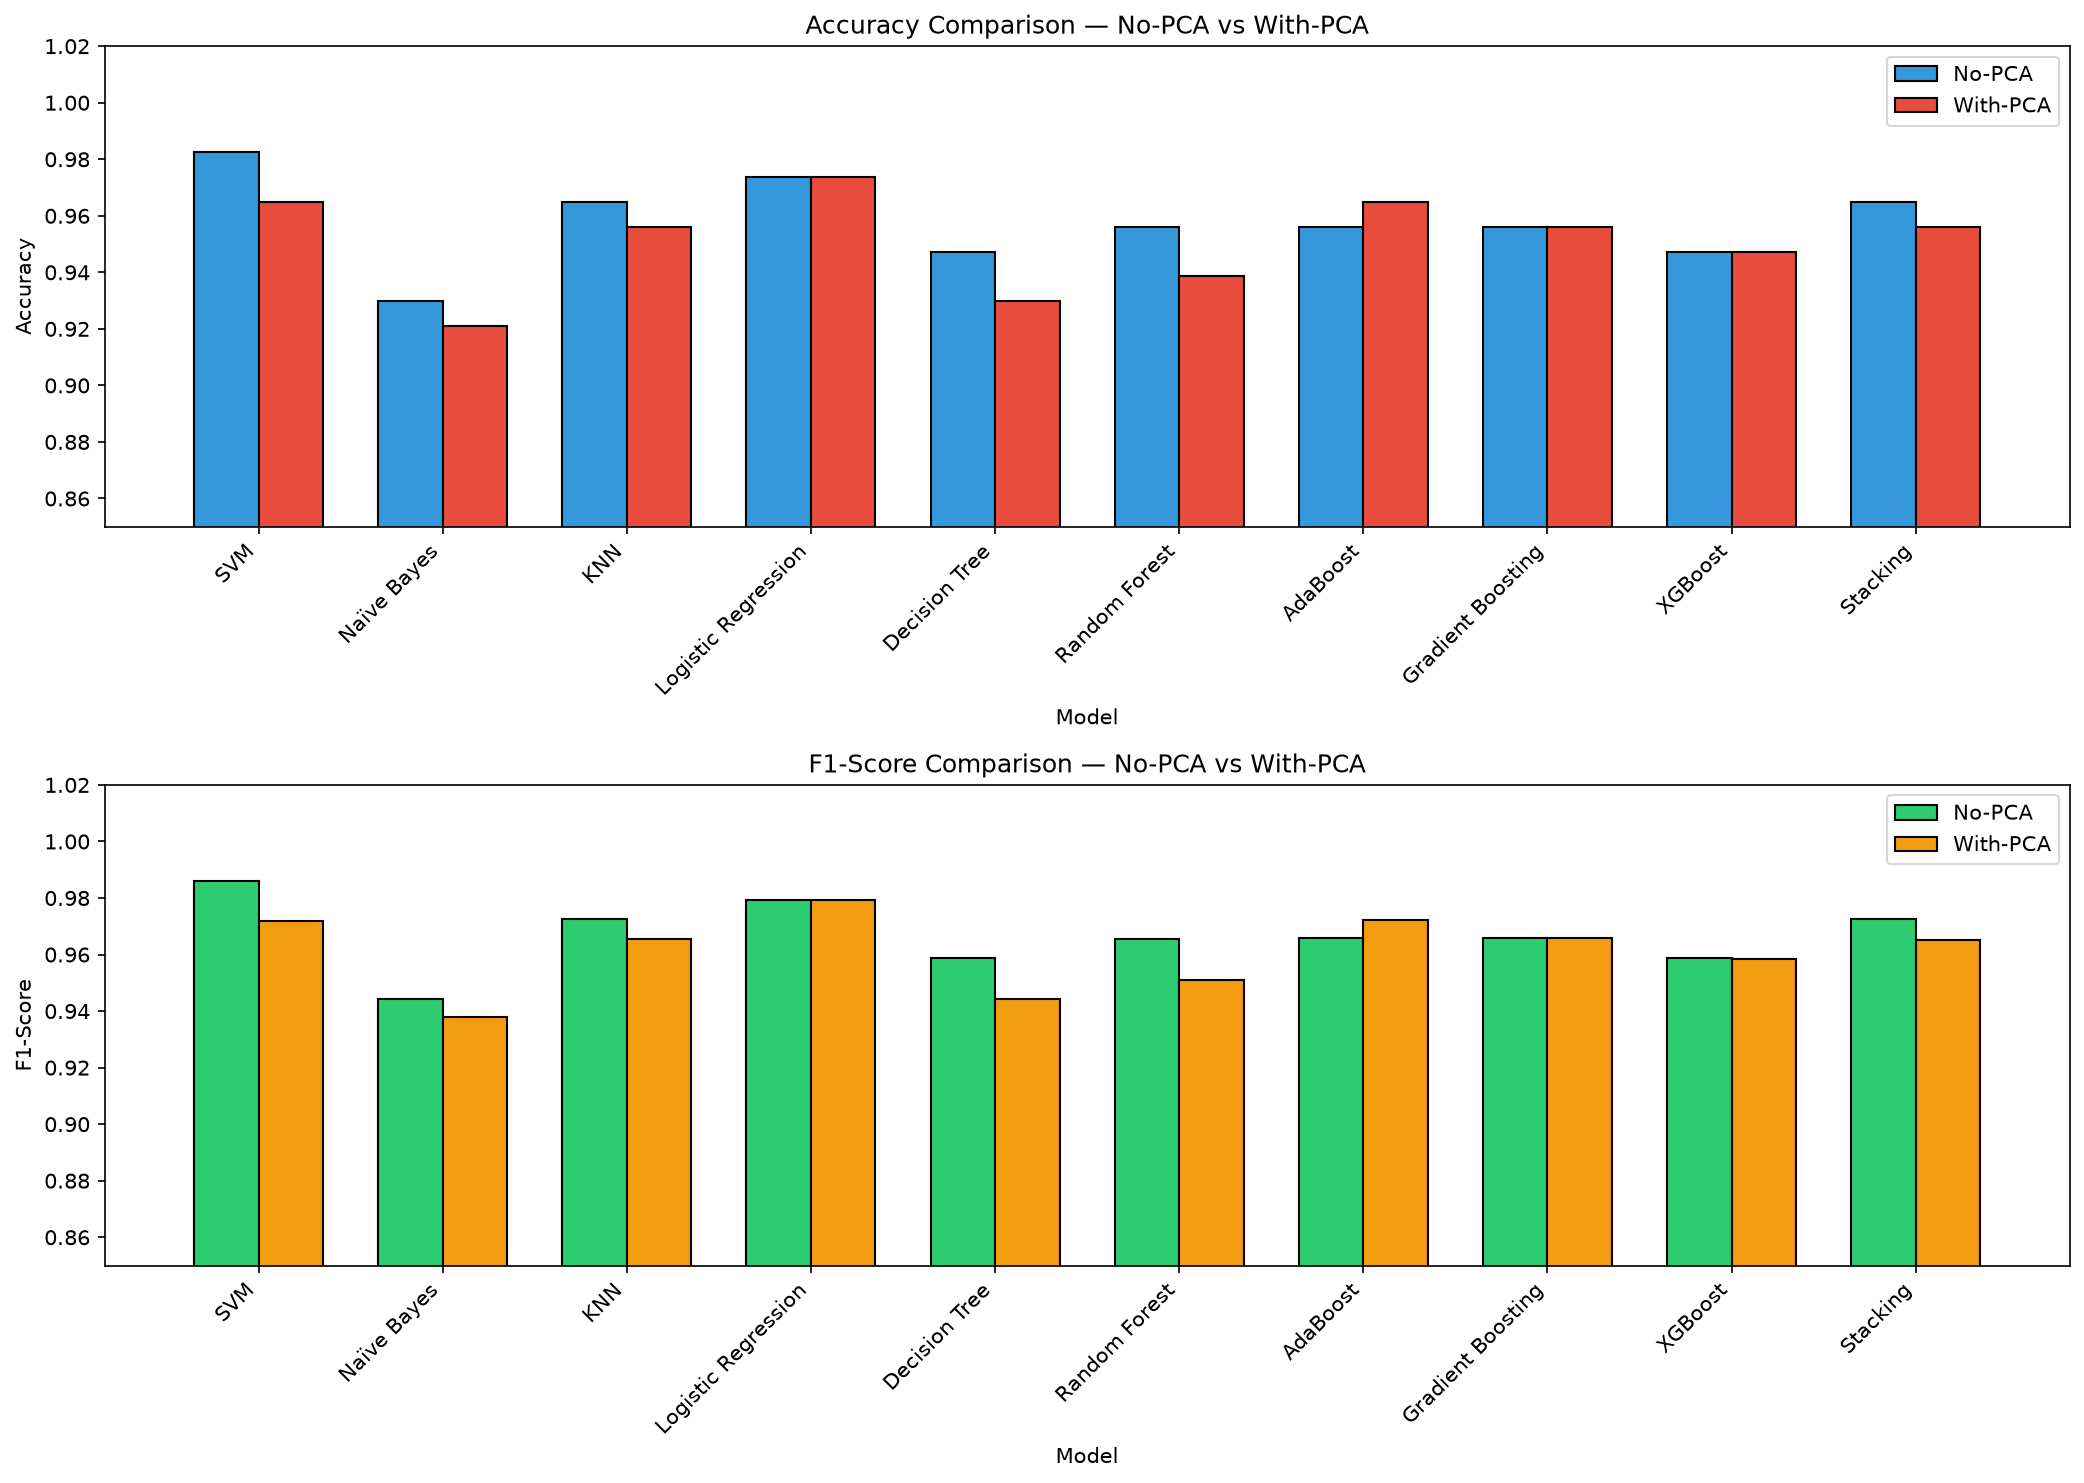
\includegraphics[width=0.85\linewidth]{images/model_comparison_barplot.png}
\caption{Accuracy and F1-Score Comparison — No-PCA vs With-PCA}
\label{fig:barplot}
\end{figure}

\textbf{Inference:}
The grouped bar charts show that most models achieve similar performance under both settings, with differences typically within 1-2 percentage points. AdaBoost is the only model that noticeably improved with PCA on this dataset, while SVM showed the largest decrease. Logistic Regression and Gradient Boosting remained unchanged, demonstrating robustness to the dimensionality reduction.

\subsection{PCA Impact Heatmap}
\begin{figure}[H]
\centering
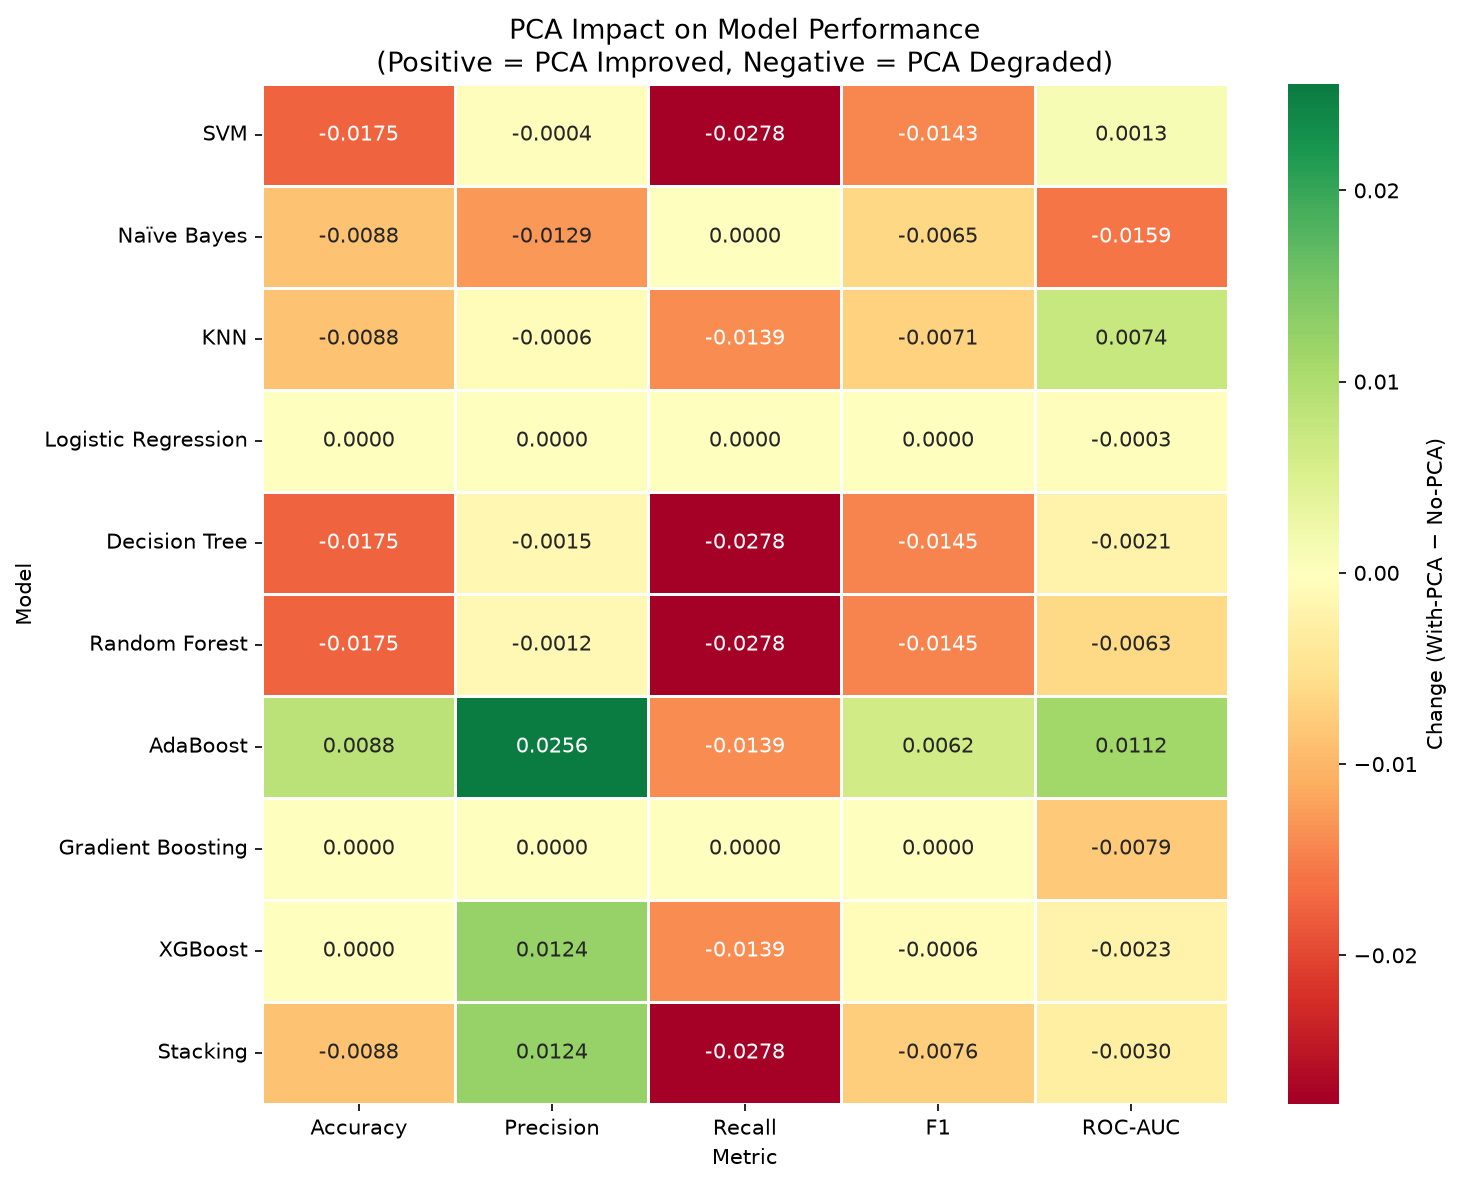
\includegraphics[width=0.75\linewidth]{images/pca_impact_heatmap.png}
\caption{PCA Impact on Model Performance (With-PCA $-$ No-PCA)}
\label{fig:impact_heatmap}
\end{figure}

\textbf{Inference:}
The heatmap quantifies the exact effect of PCA on each model-metric combination. Green cells indicate improvement, red cells indicate degradation. Logistic Regression and Gradient Boosting show near-zero changes across all metrics, while SVM and Decision Tree show consistent decreases. AdaBoost shows improvements in accuracy, precision, and AUC, suggesting that PCA removed noisy features that were interfering with its sequential learning.

\subsection{Cross-Validation Stability}
\begin{figure}[H]
\centering
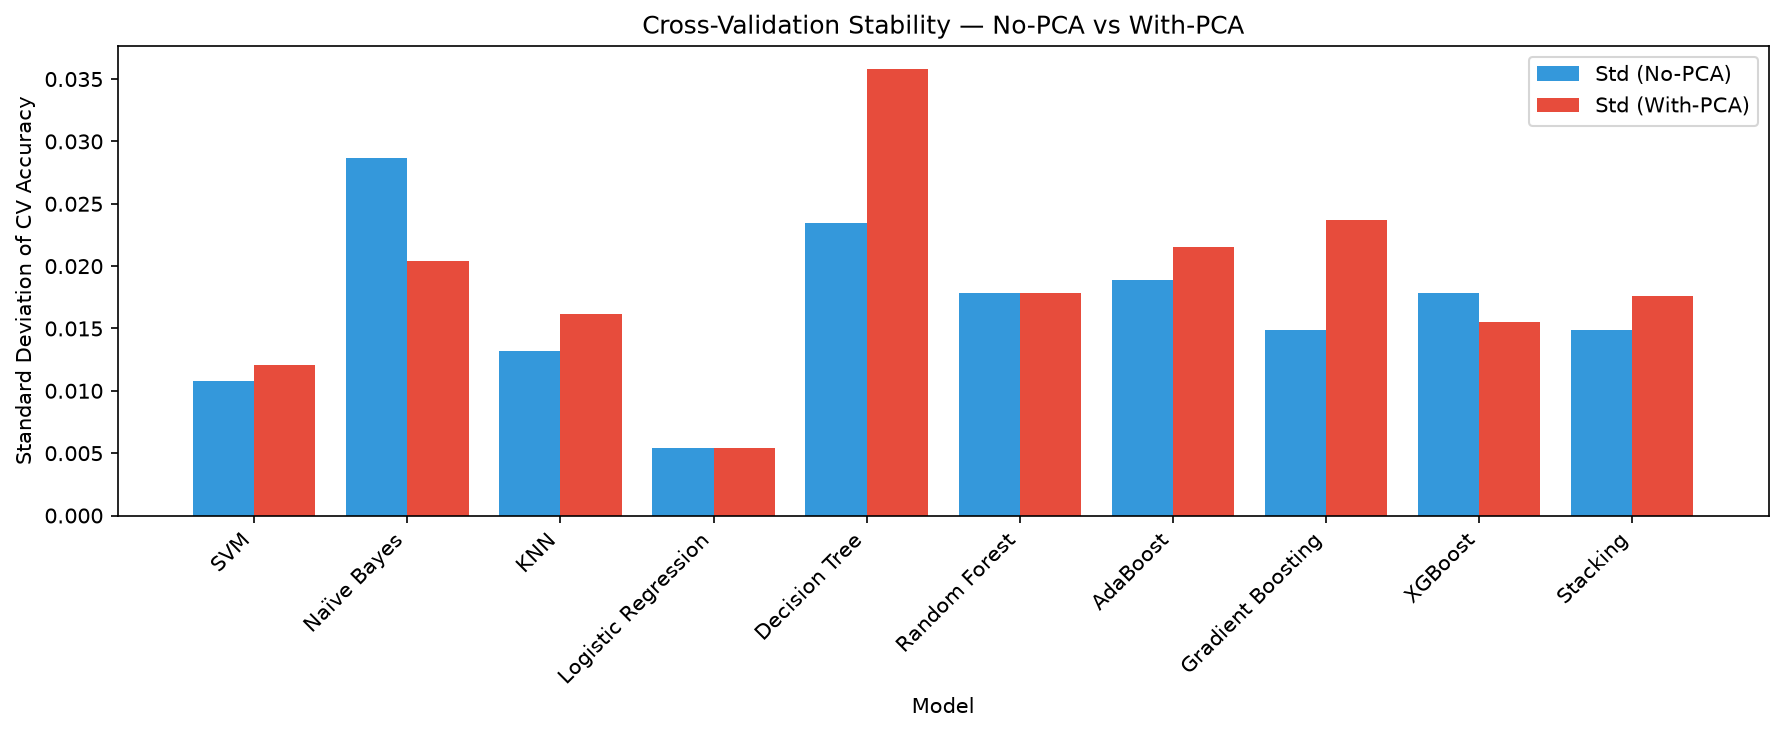
\includegraphics[width=0.85\linewidth]{images/cv_stability_comparison.png}
\caption{Cross-Validation Standard Deviation — No-PCA vs With-PCA}
\label{fig:cv_stability}
\end{figure}

\textbf{Inference:}
The standard deviation comparison reveals that PCA produced more stable predictions (lower variance) for Na\"ive Bayes and XGBoost, while slightly increasing variance for KNN, Decision Tree, and Gradient Boosting. Logistic Regression and Random Forest showed no meaningful change in stability, indicating that their performance consistency is independent of the feature space dimensionality.

\subsection{Statistical Significance Testing}

To rigorously assess whether the observed performance differences between the No-PCA and With-PCA settings are statistically significant (rather than attributable to random variation across folds), two paired statistical tests were applied to the 5-fold cross-validation accuracy scores for each model.

\textbf{Test 1 --- Paired t-test.}
The paired t-test evaluates whether the mean difference between two sets of paired observations is significantly different from zero. Given fold-wise accuracy scores $\{a_i^{\text{NP}}\}_{i=1}^{5}$ (No-PCA) and $\{a_i^{\text{WP}}\}_{i=1}^{5}$ (With-PCA), the differences $d_i = a_i^{\text{NP}} - a_i^{\text{WP}}$ are computed. The test statistic is:
\begin{equation}
t = \frac{\bar{d}}{s_d / \sqrt{n}}, \quad \text{where } \bar{d} = \frac{1}{n}\sum_{i=1}^{n} d_i, \quad s_d = \sqrt{\frac{1}{n-1}\sum_{i=1}^{n}(d_i - \bar{d})^2}
\end{equation}
Under $H_0: \mu_d = 0$, $t$ follows a Student's $t$-distribution with $n - 1 = 4$ degrees of freedom. This test assumes that the differences $d_i$ are approximately normally distributed.

\textbf{Test 2 --- Wilcoxon Signed-Rank Test.}
As a non-parametric alternative that does not assume normality (important given $n = 5$), the Wilcoxon signed-rank test is also applied. It ranks the absolute differences $|d_i|$, then computes the test statistic $W$ as the smaller of the sum of positive ranks and negative ranks:
\begin{equation}
W = \min\!\left(\sum_{d_i > 0} R_i, \;\sum_{d_i < 0} R_i\right)
\end{equation}
where $R_i$ is the rank of $|d_i|$ among all non-zero absolute differences. Under $H_0$, $W$ follows a known distribution for small $n$.

\textbf{Hypotheses and Significance Level:}
\begin{itemize}
    \item $H_0$: There is no significant difference in CV accuracy between No-PCA and With-PCA ($\mu_d = 0$).
    \item $H_1$: There is a significant difference ($\mu_d \neq 0$).
    \item Significance level: $\alpha = 0.05$.
\end{itemize}

\begin{table}[H]
\centering
\caption{Statistical Significance Testing — Paired t-test \& Wilcoxon Signed-Rank Test}
\label{tab:stat_sig}
\vspace{0.2cm}
\small
\begin{tabular}{l|cc|c|cc|cc|c}
\toprule
\textbf{Model} & \textbf{Mean} & \textbf{Mean} & \textbf{$\Delta$} & \textbf{$t$-stat} & \textbf{$p$ (t-test)} & \textbf{$W$-stat} & \textbf{$p$ (Wilcoxon)} & \textbf{Sig.?} \\
 & \textbf{(NP)} & \textbf{(WP)} & & & & & & \textbf{($\alpha$=0.05)} \\
\midrule
SVM & .9758 & .9780 & +.0022 & $-$0.5345 & 0.6213 & 2.0 & 1.0000 & No \\
Na\"ive Bayes & .9341 & .9165 & $-$.0176 & 1.7253 & 0.1596 & 2.5 & 0.2500 & No \\
KNN & .9714 & .9648 & $-$.0066 & 1.5000 & 0.2080 & 0.0 & 0.5000 & No \\
Log. Regression & .9824 & .9824 & .0000 & N/A & N/A & 0.0 & 1.0000 & No \\
Decision Tree & .9319 & .9385 & +.0066 & $-$0.4657 & 0.6657 & 6.5 & 0.9375 & No \\
Random Forest & .9626 & .9604 & $-$.0022 & 0.5345 & 0.6213 & 1.0 & 0.5000 & No \\
AdaBoost & .9802 & .9714 & $-$.0088 & 0.9300 & 0.4050 & 2.0 & 0.7500 & No \\
Grad. Boosting & .9736 & .9626 & $-$.0110 & 0.8771 & 0.4300 & 4.0 & 0.3750 & No \\
XGBoost & .9714 & .9670 & $-$.0044 & 0.2933 & 0.7839 & 3.5 & 0.7500 & No \\
Stacking & .9714 & .9758 & +.0044 & $-$1.0000 & 0.3739 & 1.0 & 0.5000 & No \\
\bottomrule
\end{tabular}
\end{table}

\textit{Note: For Logistic Regression, the paired t-test yields N/A because the 5-fold CV accuracy scores are identical under both No-PCA and With-PCA settings, resulting in zero variance in the differences.}

\begin{figure}[H]
\centering
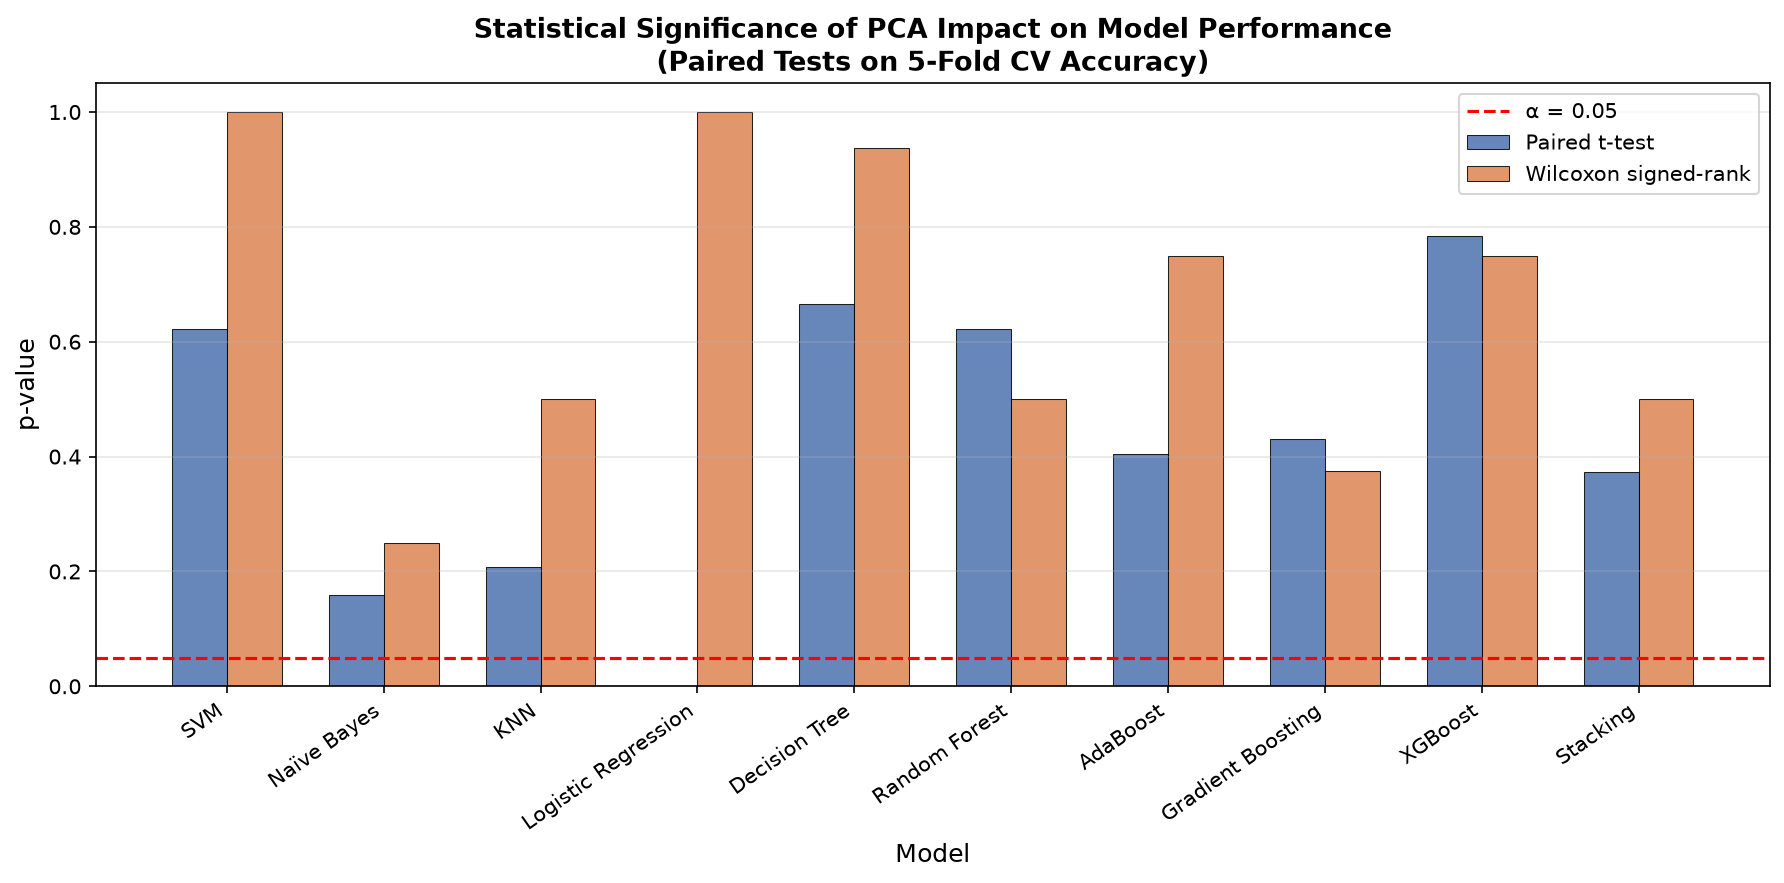
\includegraphics[width=0.85\linewidth]{images/statistical_significance.png}
\caption{Statistical Significance of PCA Impact — $p$-values from Paired t-test and Wilcoxon Signed-Rank Test (Red dashed line: $\alpha = 0.05$)}
\label{fig:stat_sig}
\end{figure}

\textbf{Inference:}
None of the 10 models show a statistically significant difference between No-PCA and With-PCA cross-validation accuracy at $\alpha = 0.05$. The closest to significance is Na\"ive Bayes ($t = 1.7253$, $p = 0.1596$), which had the largest absolute accuracy gap ($\Delta = -1.76$ percentage points), yet still does not cross the significance threshold. Logistic Regression yields identical fold scores under both settings, making the paired $t$-test undefined (N/A). All other models produce $p$-values well above 0.05, indicating that the observed differences are within the range of normal fold-to-fold variation. This outcome is expected given the low statistical power inherent to $n = 5$ paired observations --- small but real effects are unlikely to reach significance. The Wilcoxon signed-rank test corroborates the $t$-test results across all models. These findings confirm that while descriptive performance differences exist between the two feature spaces, none are large enough to be declared statistically significant with 5-fold cross-validation.

\section{Discussion}

\subsection{Observation Questions}

\begin{enumerate}
    \item \textbf{Which models improved most with PCA? Which did not? Why?}\\
    AdaBoost was the only model that showed a clear accuracy improvement with PCA ($+0.88$ percentage points on the test set). Its ROC-AUC also improved from 0.9818 to 0.9931. This improvement occurred because PCA removed noisy, redundant features that were causing the weak learners to overfit to irrelevant patterns. In contrast, SVM showed the largest decrease ($-1.75$ pp) because its optimal linear decision boundary in the full 30-dimensional space was slightly less effective in the 10-component PCA space. Decision Tree and Random Forest also declined, as these models rely on individual feature splits and PCA's linear combinations obscured the original axis-aligned thresholds they depend on.

    \item \textbf{Did PCA reduce variance across folds (more stable results)?}\\
    PCA reduced fold-to-fold variance for Na\"ive Bayes (std: 0.0287 $\to$ 0.0204) and XGBoost (std: 0.0179 $\to$ 0.0155). For Na\"ive Bayes, this occurred because PCA produces uncorrelated components, which better satisfies the feature independence assumption and leads to more consistent predictions. However, several models showed slightly increased variance with PCA (KNN, Decision Tree, AdaBoost, Gradient Boosting), suggesting that the reduced feature space introduced additional sensitivity to fold composition for these algorithms.

    \item \textbf{For high-dimensional data, was PCA beneficial in reducing overfitting?}\\
    With 30 features and 569 samples, the WDBC dataset is moderately high-dimensional. PCA compressed the feature space from 30 to 10 components while retaining 95.27\% of variance. The cross-validation averages show that Decision Tree (93.19\% $\to$ 93.85\%) and Stacking (97.14\% $\to$ 97.58\%) had higher CV accuracy with PCA, suggesting reduced overfitting for these models. However, the overall impact on overfitting was modest, likely because the dataset does not have an extreme dimensionality-to-sample-size ratio.

    \item \textbf{How did linear models behave compared to ensemble models with PCA?}\\
    Logistic Regression showed perfect stability: identical performance (97.37\% accuracy, 0.9793 F1) under both settings, indicating it is robust to the dimensionality change at this variance threshold. SVM with a linear kernel decreased slightly ($-1.75$ pp). Among ensemble models, Gradient Boosting and XGBoost remained unchanged in test accuracy, while Random Forest decreased ($-1.75$ pp). The key distinction is that linear models benefit from PCA's removal of multicollinearity (which can destabilize coefficient estimates), while tree-based ensembles are naturally robust to multicollinearity but may lose useful axis-aligned splitting information after PCA's linear transformation.

    \item \textbf{Did Stacking show robustness to dimensionality reduction compared to single models?}\\
    Stacking demonstrated moderate robustness, with a test accuracy change of only $-0.88$ pp (96.49\% $\to$ 95.61\%) and a CV accuracy improvement of $+0.44$ pp (97.14\% $\to$ 97.58\%). The meta-learner was able to compensate when individual base learners lost performance, because different base models responded differently to PCA. For comparison, the average single-model accuracy change was $-0.61$ pp, indicating that Stacking's performance shift was comparable to the average individual model.
\end{enumerate}

\section{Conclusion}
Ten machine learning classifiers were trained and evaluated on the Wisconsin Diagnostic Breast Cancer dataset under two conditions: using all 30 original standardized features (No-PCA) and using 10 PCA components retaining 95.27\% of variance (With-PCA). Hyperparameter tuning with 5-fold stratified cross-validation was performed for every model under both settings.

The highest No-PCA test accuracy was achieved by \textbf{SVM} at \textbf{98.25\%}, while \textbf{Logistic Regression} achieved the highest With-PCA test accuracy at \textbf{97.37\%}. Logistic Regression also demonstrated the best cross-validation consistency (CV accuracy: 98.24\%) under both conditions.

The results show that PCA's impact is model-dependent: it improved AdaBoost (by removing noisy features), left Logistic Regression, Gradient Boosting, and XGBoost essentially unchanged, and slightly reduced performance for SVM, Decision Tree, and Random Forest. This confirms that PCA is most beneficial when the model is sensitive to multicollinearity or high-dimensional noise, and less impactful for models with built-in feature selection or regularization mechanisms.

\section{References}
\begin{enumerate}[label={[\arabic*]}]
    \item Scikit-learn Documentation. \textit{Decomposition: PCA}. \url{https://scikit-learn.org/stable/modules/decomposition.html#pca}
    \item Scikit-learn Documentation. \textit{Ensemble methods}. \url{https://scikit-learn.org/stable/modules/ensemble.html}
    \item Scikit-learn Documentation. \textit{Breast Cancer Wisconsin (Diagnostic) Dataset}. \url{https://scikit-learn.org/stable/datasets/toy_dataset.html#breast-cancer-dataset}
    \item Jolliffe, I. T. (2002). \textit{Principal Component Analysis}. Springer Series in Statistics, 2nd Ed.
    \item Chen, T., \& Guestrin, C. (2016). \textit{XGBoost: A Scalable Tree Boosting System}. Proceedings of the 22nd ACM SIGKDD Conference.
\end{enumerate}

\end{document}
